% !TeX program = pdfLaTeX
\documentclass[12pt]{article}
\usepackage{amsmath}
\usepackage{graphicx,psfrag,epsf}
\usepackage{enumerate}
\usepackage{natbib}
\usepackage{textcomp}
\usepackage[hyphens]{url} % not crucial - just used below for the URL
\usepackage{hyperref}
\providecommand{\tightlist}{%
  \setlength{\itemsep}{0pt}\setlength{\parskip}{0pt}}

%\pdfminorversion=4
% NOTE: To produce blinded version, replace "0" with "1" below.
\newcommand{\blind}{0}

% DON'T change margins - should be 1 inch all around.
\addtolength{\oddsidemargin}{-.5in}%
\addtolength{\evensidemargin}{-.5in}%
\addtolength{\textwidth}{1in}%
\addtolength{\textheight}{1.3in}%
\addtolength{\topmargin}{-.8in}%

%% load any required packages here



% Pandoc citation processing

\newcommand{\ear}[1]{{\textcolor{blue}{#1}}}
\newcommand{\svp}[1]{{\textcolor{RedOrange}{#1}}}
\newcommand{\rh}[1]{{\textcolor{Green}{#1}}}
\usepackage[capitalise]{cleveref}
\newcommand\pcref[1]{(\cref{#1})}
\usepackage{algorithm,algpseudocode,booktabs}

\begin{document}


\def\spacingset#1{\renewcommand{\baselinestretch}%
{#1}\small\normalsize} \spacingset{1}


%%%%%%%%%%%%%%%%%%%%%%%%%%%%%%%%%%%%%%%%%%%%%%%%%%%%%%%%%%%%%%%%%%%%%%%%%%%%%%

\if0\blind
{
  \title{\bf Eye Fitting Straight Lines in the Modern Era}

  \author{
        Emily A. Robinson 1 \\
    Department of Statistics, University of Nebraska - Lincoln\\
     and \\     Susan VanderPlas 2 \\
    Department of Statistics, University of Nebraska - Lincoln\\
     and \\     Reka Howard 3 \\
    Department of Statistics, University of Nebraska - Lincoln\\
      }
  \maketitle
} \fi

\if1\blind
{
  \bigskip
  \bigskip
  \bigskip
  \begin{center}
    {\LARGE\bf Eye Fitting Straight Lines in the Modern Era}
  \end{center}
  \medskip
} \fi

\bigskip
\begin{abstract}
Fitting lines by eye through a set of points has been explored since the
20th century. Common methods of fitting trends by eye involve
maneuvering a string, black thread, or ruler until the fit is suitable,
then drawing the line through the set of points. In 2015, the New York
Times introduced an interactive feature, called `You Draw It'. Readers
are asked to input their own assumptions about various metrics and
compare how these assumptions relate to reality. The New York Times team
utilizes Data Driven Documents (D3) that allows readers to predict these
metrics by drawing a line on their computer screen with their computer
mouse. In my research, I established `You Draw It' as a method for
graphical testing by adapting the New York Times feature. I recruited
participants via crowdsourcing websites and replicated the study found
in Eye Fitting Straight Lines (Mosteller et al., 1981). Participants
were directed to an RShiny application link and shown points following a
linear trend and asked to draw a line through the data points using
their computer mouse; task plots were generated using the r2d3 package
in R statistical software. Results from my study were consistent with
those found in the previous study; when shown points following a linear
trend, participants tended to fit the slope of the first principal
component over the slope of the least-squares regression line. This
trend was most prominent when shown data simulated with larger
variances. The reproducibility of these results serves as evidence of
the reliability of the you draw it method. Future work is necessary to
implement the `You Draw It' tool as a method of testing graphics. {[}200
word limit{]}
\end{abstract}

\noindent%
{\it Keywords:} Graphics, Regression, Graph
Perception, Scatterplot, Cognitive Bias
\vfill

\newpage
\spacingset{1.45} % DON'T change the spacing!

\hypertarget{introduction}{%
\section{Introduction}\label{introduction}}

Advanced technology and computing power have promoted data visualization
as a central tool in modern data science. \citet{unwin2020data} defines
data visualization as the art of drawing graphical charts in order to
display data. Graphics are useful for data cleaning, exploring data
structure, and have been an essential component in communicating
information for the last 200 years \citep{lewandowsky1989perception}.
Although statistical graphics have become widely used and valued in
science, business, and in many other aspects of life, as creators of
graphics, we are too accepting of them as default without asking
critical questions about the graphics we create or view (Unwin, 2020).

\hypertarget{graph-perception}{%
\subsection{Graph Perception}\label{graph-perception}}

\hypertarget{testing-statistical-graphics}{%
\subsection{Testing Statistical
Graphics}\label{testing-statistical-graphics}}

One way in which we evaluate the effectiveness of charts is through the
use of graphical tests. We could ask participants to identify
differences in graphs, read information off of a chart accurately, use
data to make correct real-world decisions, or predict the next few
observations. All of these types of tests require different levels of
use and manipulation of the information being presented in the chart.

\begin{itemize}
\tightlist
\item
  Psychophysics (speed and accuracy)
\item
  Lineups
\end{itemize}

\hypertarget{trend-judgement}{%
\subsection{Trend Judgement}\label{trend-judgement}}

\begin{itemize}
\tightlist
\item
  \citet{finney1951subjective}
\item
  \citet{mosteller_eye_1981}
\item
  \citet{ciccione2021can}
\end{itemize}

Initial studies in the 20th century explored the use of fitting lines by
eye through a set of points
\citep{finney1951subjective, mosteller_eye_1981}. Common methods of
fitting trends by eye involve maneuvering a string, black thread, or
ruler until the fit is suitable, then drawing the line through the set
of points. In \citet{finney1951subjective}, it was of interest to
determine the effect of stopping iterative maximum likelihood
calculations after one iteration. Many techniques in statistical
analysis are performed with the aid of iterative calculations such as
Newton's method or Fisher's scoring. Guesses are made at the best
estimates of certain parameters and these guesses are then used as the
basis of a computation which yields a new set of approximation to the
parameter estimates; this same procedure is the performed on the new
parameter estimates and the computing cycle is repeated until
convergence, as determined by the statistician, is reached. The author
was interested in whether one iteration of calculations was sufficient
in the estimation of parameters connected with dose-response
relationships. One measure of interest is the relative potency between a
test preparation of doses and standard preparation of does; relative
potency is calculated as the ratio of two equally effective doses
between the two preparation methods. \cref{fig:subjective-judgement}
shows a pair of parallel probit responses in a biological assay. The
x-axis is the \(\log_{1.5}\) dose level for four dose levels (for
example, doses 4, 6, 9, and 13 correspond correspond to equally spaced
values on a logarithmic scale, labeled 0, 1, 2, and 3) and the y-axis is
the corresponding probit response as calculated in
\citet{finney1948table}; circles correspond to the test preparation
method while the crosses correspond to the standard preparation method.
For these sort of assays, the does-response relationship follows a
linear regression of the probit response on the logarithm of the dose
levels; the two preparation methods can be constrained to be parallel
\citep{jerne1949validity}, limiting the relative potency to one
consistent value. In this study, twenty-one scientists were recruited
via postal mail and asked to ``rule two lines'' in order to judge by eye
the positions for a pair of parallel probit regression lines in a
biological assay. The author then computed one iterative calculation of
the relative potency based on starting values as indicated by the pair
of lines provided by each participant and compared these relative
potency estimates to that which was estimated by the full probit
technique (reaching convergence through multiple iterations). Results
indicated that one cycle of iterations for calculating the relative
potency was sufficient based on the starting values provided by eye from
the participants.

Thirty years later, Mosteller et al.~(1981), sought to understand the
properties of least squares and other computed lines by establishing one
systematic method of fitting lines by eye. The authors recruited 153
graduate students and post doctoral researchers in Introductory
Biostatistics. Participants were asked to fit lines by eye to four
scatterplots using an 8.5 x 11 inch transparency with a straight line
etched completely across the middle. A latin square design
\citep{giesbrecht2004planning} with packets of the set of points stapled
together in four different sequences was used to determine if there is
an effect of order of presentation. It was found that order of
presentation had no effect and that participants tended to fit the slope
of the first principal component (error minimized orthogonally, both
horizontal and vertical, to the regression line) over the slope of the
least squares regression line (error minimized vertically to the
regression line).

In 2015, the New York Times introduced an interactive feature, called
You Draw It
\citep{aisch_cox_quealy_2015, buchanan_park_pearce_2017, katz_2017}.
Readers are asked to input their own assumptions about various metrics
and compare how these assumptions relate to reality. The New York Times
team utilizes Data Driven Documents (D3) that allows readers to predict
these metrics through the use of drawing a line on their computer screen
with their computer mouse. \citep{katz_2017} is one such example in
which readers are asked to draw the line for the missing years providing
what they estimate to be the number of Americans who have died every
year from car accidents, since 1990. After the reader has completed
drawing the line, the actual observed values are revealed and the reader
may check their estimated knowledge against the actual reported data.

Major news and research organizations such as the New York Times,
FiveThirtyEight, Washington Post, and the Pew Research Center create and
customize graphics with Data Driven Documents (D3). In June 2020, the
New York Times released a front page displaying figures that represent
each of the 100,000 lives lost from the COVID-19 pandemic until this
point in time \citep{NYTrememberinglives}; this visualization was meant
to bring about a visceral reaction and resonate with readers. During
2021 March Madness, FiveThirtyEight created a roster-shuffling machine
which allowed readers to build their own NBA contender through
interactivity \citep{ryanabest_2021}. Data Driven Documents (D3) is an
open-source JavaScript based graphing framework created by Mike Bostock
during his time working on graphics at the New York Times. For readers
familiar with R, it is notable to consider D3 in JavaScript equivalent
to the ggplot2 package in R \citep{ggplot2}.

\hypertarget{research-objective}{%
\subsection{Research objective}\label{research-objective}}

The goal of this paper is to establish you draw it as a tool for
measuring predictions of trends fitted by eye and a method for testing
graphics. In order to validate you draw it as a method for testing
graphics, the first sub-study, referred to as Eye Fitting Straight Lines
in the Modern Era, replicated the experiment and results found in
Mosteller et al.~(1981).

\hypertarget{study-development}{%
\section{Study Development}\label{study-development}}

\hypertarget{interactive-plot-development}{%
\subsection{Interactive Plot
Development}\label{interactive-plot-development}}

\hypertarget{data-generation}{%
\subsection{Data Generation}\label{data-generation}}

All data processing was conducted in R before being passed to the D3.js
source code. A total of \(N = 30\) points \((x_i, y_i), i = 1,...N\)
were generated for \(x_i \in [x_{min}, x_{max}]\) where \(x\) and \(y\)
have a linear relationship. Data were simulated based on linear model
with additive errors: \begin{align}
y_i & = \beta_0 + \beta_1 x_i + e_i \\
\text{with } e_i & \sim N(0, \sigma^2). \nonumber
\end{align} The parameters \(\beta_0\) and \(\beta_1\) are selected to
replicate Mosteller et al.~(1981) with \(e_i\) generated by rejection
sampling in order to guarantee the points shown align with that of the
fitted line. An ordinary least squares regression is then fit to the
simulated points in order to obtain the best fit line and fitted values
in 0.25 increments across the domain,
\((x_k, \hat y_{k,OLS}), k = 1, ..., 4 x_{max} +1\). The data simulation
function then outputs a list of point data and line data both indicating
the parameter identification, x-value, and corresponding simulated or
fitted y value. The data simulation procedure is described in
\cref{alg:eyefitting-algorithm}.

\begin{algorithm}
  \caption{Eye Fitting Straight Lines in the Modern Era Data Simulation}\label{alg:eyefitting-algorithm}
  \begin{algorithmic}[1]
    \Statex \textbullet~\textbf{Input Parameters:} $y_{\bar{x}}$ for calculating the y-intercept, $\beta_0$; slope $\beta_1$; standard deviation from line $\sigma$; sample size of points $N = 30$; domain $x_{min}$ and $x_{max}$; fitted value increment $x_{by} = 0.25$.
    \Statex \textbullet~\textbf{Output Parameters:} List of point data and line data each indicating the parameter identification, x value, and corresponding simulated or fitted y value.
    \State Randomly select and jitter $N = 30$ x-values along the domain, $x_{i=1:N}\in [x_{min}, x_{max}]$.
    \State Determine the y-intercept, $\beta_0$, at x = 0 from the provided slope ($\beta_1$) and y-value at the mean of x ($y_{\bar{x}}$) using point-slope equation of a line.
    \State Generate "good" errors, $e_{i = 1:N}$ based on $N(0,\sigma)$ by setting a constraint requiring the mean of the first $\frac{1}{3}\text{N}$ errors $< |2\sigma|.$
    \State Simulate point data based on $y_i = \beta_0 + \beta_1 x_i + e_i$
    \State Obtain ordinary least squares regression coefficients, $\hat\beta_0$ and $\hat\beta_1$, for the simulated point data using the lm function in the stats package in base R.
    \State Obtain fitted values every 0.25 increment across the domain from the ordinary least squares regression $\hat y_{k,OLS} = \hat\beta_{0,OLS} + \hat\beta_{1,OLS} x_k$.
    \State Output data list of point data and line data each indicating the parameter identification, x value, and corresponding simulated or fitted y value.
  \end{algorithmic}
\end{algorithm}

\begin{table}

\caption{\label{tab:eyefitting-parameters}Eye Fitting Straight Lines in the Modern Era simulation model parameters}
\centering
\begin{tabular}[t]{cccc}
\toprule
Parameter Choice & $y_{\bar{x}}$ & $\beta_1$ & $\sigma$\\
\midrule
S & 3.88 & 0.66 & 1.30\\
F & 3.90 & 0.66 & 1.98\\
V & 3.89 & 1.98 & 1.50\\
N & 4.11 & -0.70 & 2.50\\
\bottomrule
\end{tabular}
\end{table}

Simulated model equation parameters were selected to reflect the four
data sets (F, N, S, and V) used in \citet{mosteller_eye_1981}
(\cref{tab:eyefitting-parameters}). Parameter choices F, N, and S
simulated data across a domain of 0 to 20. Parameter choice F produces a
trend with a positive slope and a large variance while N has a negative
slope and a large variance. In comparison, S shows a trend with a
positive slope with a small variance and V yields a steep positive slope
with a small variance over the domain of 4 to 16.
\cref{fig:eyefitting-simplot} illustrates an example of simulated data
for all four parameter choices intended to reflect the trends seen in
\cref{fig:mosteller-eyefitting-plot}. Aesthetic design choices were made
consistent across each of the interactive you draw it plots; the aspect
ratio, defining the \(x\) to \(y\) axis ratio was set to one and the
y-axis range extended 10\% beyond (above and below) the range of the
simulated data points to allow for users to draw outside the simulated
data set range.

\begin{figure}[tbp]

{\centering 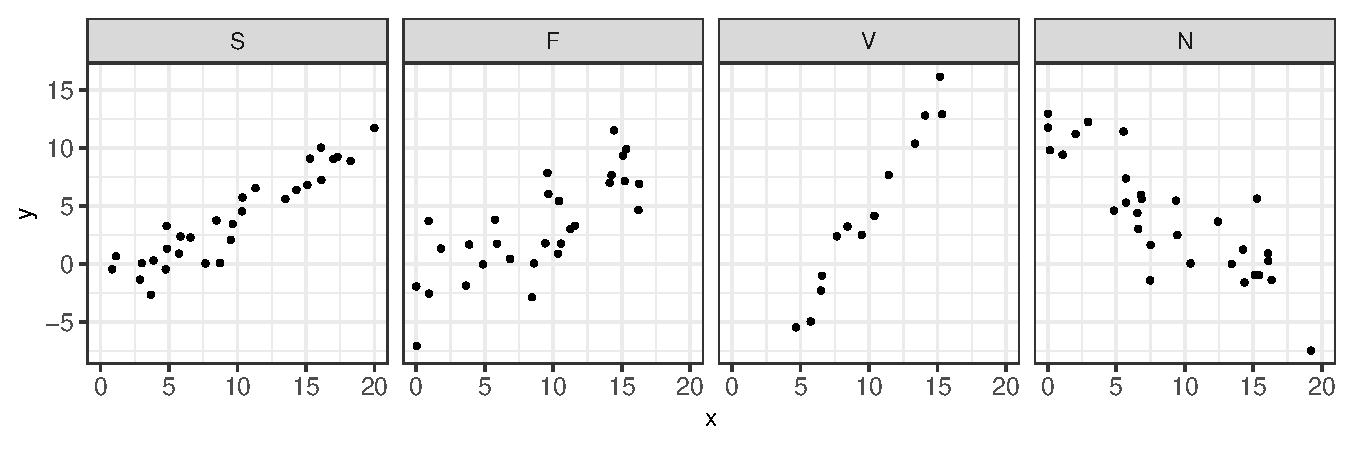
\includegraphics[width=0.75\linewidth,]{Eye-Fitting-Stright-Lines-in-the-Modern-Era_files/figure-latex/eyefitting-simplot-1} 

}

\caption{Eye Fitting Straight Lines in the Modern Era Simulated Data Example}\label{fig:eyefitting-simplot}
\end{figure}

\hypertarget{study-design}{%
\subsection{Study Design}\label{study-design}}

Participants completed the experiment using a RShiny application found
\href{https://shiny.srvanderplas.com/you-draw-it/}{here}. During May
2021, participants were recruited through Twitter, Reddit, and direct
email. A total of 39 individuals completed 256 unique you draw it task
plots; all completed you draw it task plots were included in the
analysis.

\hypertarget{results}{%
\section{Results}\label{results}}

In addition to the participant drawn points, \((x_k, y_{k,drawn})\), and
the ordinary least squares (OLS) regression fitted values,
\((x_k, \hat y_{k,OLS})\), a regression equation with a slope based on
the first principal component (PCA) was used to calculate fitted values,
\((x_k, \hat y_{k,PCA})\). For each set of simulated data and parameter
choice, the PCA regression equation was determined by using the princomp
function in the stats package in base R to obtain the rotation of the
coordinate axes from the first principal component (direction which
captures the most variance). The estimated slope, \(\hat\beta_{1,PCA}\),
is determined by the ratio of the axis rotation in y and axis rotation
in x of the first principal component with the y-intercept,
\(\hat\beta_{0,PCA}\) calculated by the point-slope equation of a line
using the mean of of the simulated points, \((\bar x_i, \bar y_i)\).
Fitted values, \(\hat y_{k,PCA}\) are then obtained every 0.25 increment
across the domain from the PCA regression equation,
\(\hat y_{k,PCA} = \hat\beta_{0,PCA} + \hat\beta_{1,PCA} x_k\).
\cref{fig:ols-vs-pca-example} illustrates the difference between an OLS
regression equation which minimizes the vertical distance of points from
the line and a regression equation with a slope calculated by the first
principal component which minimizes the smallest distance of points from
the line.

\begin{figure}[tbp]

{\centering 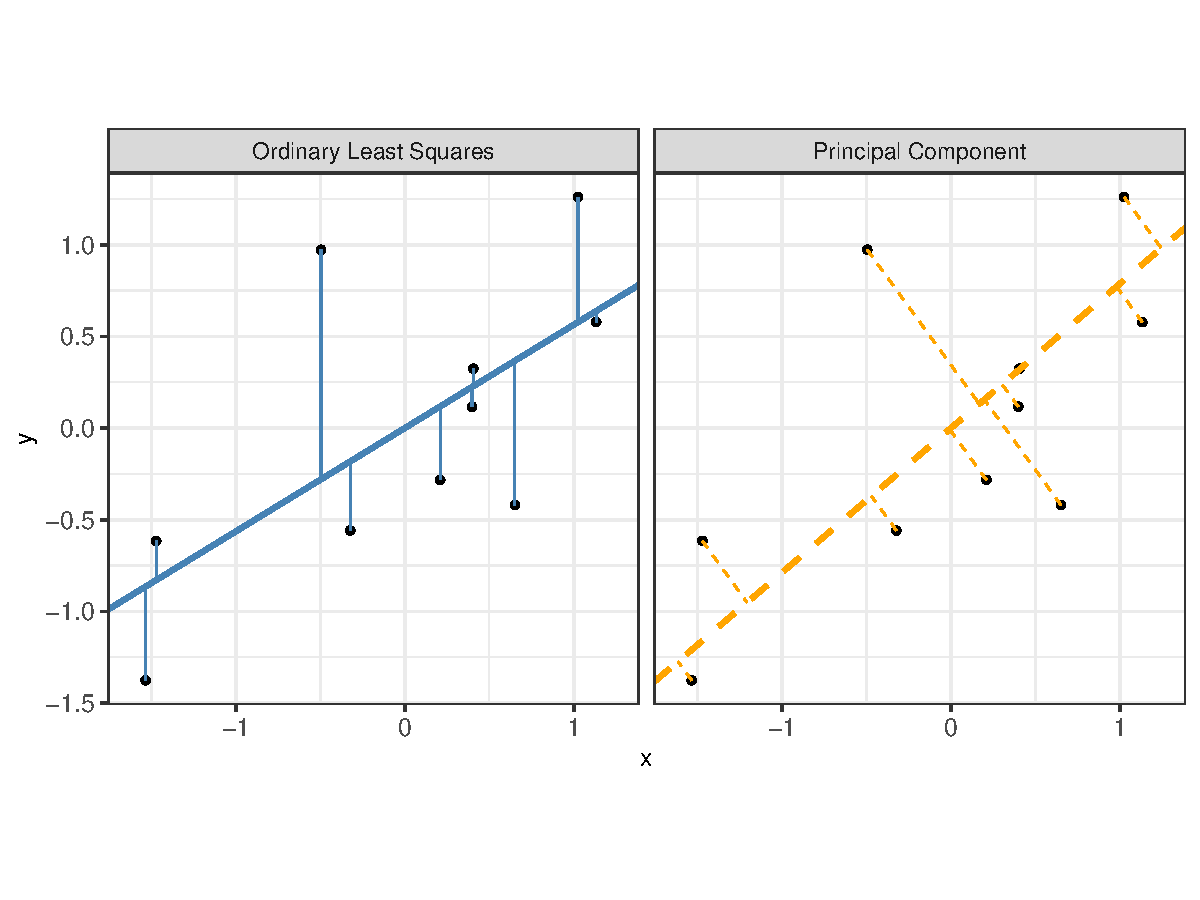
\includegraphics[width=1\linewidth,]{Eye-Fitting-Stright-Lines-in-the-Modern-Era_files/figure-latex/ols-vs-pca-example-1} 

}

\caption{OLS vs PCA Regression Lines}\label{fig:ols-vs-pca-example}
\end{figure}

For each participant, the final data set used for analysis contains
\(x_{ijk}, y_{ijk,drawn}, \hat y_{ijk,OLS}\), and \(\hat y_{ijk,PCA}\)
for parameter choice \(i = 1,2,3,4\), j = \(1,...N_{participant}\), and
\(x_{ijk}\) value \(k = 1, ...,4 x_{max} + 1\). Using both a linear
mixed model and a generalized additive mixed model, comparisons of
vertical residuals in relation to the OLS fitted values
(\(e_{ijk,OLS} = y_{ijk,drawn} - \hat y_{ijk,OLS}\)) and PCA fitted
values (\(e_{ijk,PCA} = y_{ijk,drawn} - \hat y_{ijk,PCA}\)) were made
across the domain. \cref{fig:eyefitting-example-plot} displays an
example of all three fitted trend lines for parameter choice F.

\begin{figure}[tbp]

{\centering 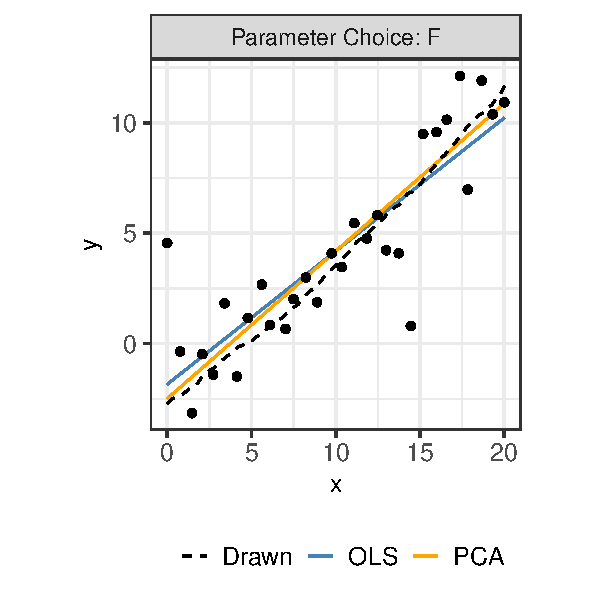
\includegraphics[width=0.65\linewidth,]{Eye-Fitting-Stright-Lines-in-the-Modern-Era_files/figure-latex/eyefitting-example-plot-1} 

}

\caption{Eye Fitting Straight Lines in the Modern Era Example}\label{fig:eyefitting-example-plot}
\end{figure}

Using the lmer function in the lme4 package \citep{lme4}, a linear mixed
model (LMM) is fit separately to the OLS and PCA residuals, constraining
the fit to a linear trend. Parameter choice, \(x\), and the interaction
between \(x\) and parameter choice were treated as fixed effects with a
random participant effect accounting for variation due to participant.
The LMM equation for each fit (OLS and PCA) residuals is given by:
\begin{equation}
y_{ijk,drawn} - \hat y_{ijk,fit} = e_{ijk,fit} = \left[\gamma_0 + \alpha_i\right] + \left[\gamma_{1} x_{ijk} + \gamma_{2i} x_{ijk}\right] + p_{j} + \epsilon_{ijk}
\end{equation} \noindent where

\begin{itemize}
\tightlist
\item
  \(y_{ijk,drawn}\) is the drawn y-value for the \(i^{th}\) parameter
  choice, \(j^{th}\) participant, and \(k^{th}\) increment of x-value
\item
  \(\hat y_{ijk,fit}\) is the fitted y-value for the \(i^{th}\)
  parameter choice, \(j^{th}\) participant, and \(k^{th}\) increment of
  x-value corresponding to either the OLS or PCA fit
\item
  \(e_{ijk,fit}\) is the residual between the drawn and fitted y-values
  for the \(i^{th}\) parameter choice, \(j^{th}\) participant, and
  \(k^{th}\) increment of x-value corresponding to either the OLS or PCA
  fit
\item
  \(\gamma_0\) is the overall intercept
\item
  \(\alpha_i\) is the effect of the \(i^{th}\) parameter choice (F, S,
  V, N) on the intercept
\item
  \(\gamma_1\) is the overall slope for \(x\)
\item
  \(\gamma_{2i}\) is the effect of the parameter choice on the slope
\item
  \(x_{ijk}\) is the x-value for the \(i^{th}\) parameter choice,
  \(j^{th}\) participant, and \(k^{th}\) increment
\item
  \(p_{j} \sim N(0, \sigma^2_{participant})\) is the random error due to
  the \(j^{th}\) participant's characteristics
\item
  \(\epsilon_{ijk} \sim N(0, \sigma^2)\) is the residual error.
\end{itemize}

Eliminating the linear trend constraint, the bam function in the mgcv
package \citep{mgcv1, mgcv2, mgcv3, mgcv4, mgcv5} is used to fit a
generalized additive mixed model (GAMM) separately to the OLS and PCA
residuals to allow for estimation of smoothing splines. Parameter choice
was treated as a fixed effect with no estimated intercept and a separate
smoothing spline for \(x\) was estimated for each parameter choice. A
random participant effect accounting for variation due to participant
and a random spline for each participant accounted for variation in
spline for each participant. The GAMM equation for each fit (OLS and
PCA) residuals is given by: \begin{equation}
y_{ijk, drawn} - \hat y_{ijk, fit} = e_{ijk,fit} = \alpha_i + s_{i}(x_{ijk}) + p_{j} + s_{j}(x_{ijk})
\end{equation} \noindent where

\begin{itemize}
\tightlist
\item
  \(y_{ijk,drawn}\) is the drawn y-value for the \(i^{th}\) parameter
  choice, \(j^{th}\) participant, and \(k^{th}\) increment of x-value
\item
  \(\hat y_{ijk,fit}\) is the fitted y-value for the \(i^{th}\)
  parameter choice, \(j^{th}\) participant, and \(k^{th}\) increment of
  x-value corresponding to either the OLS or PCA fit
\item
  \(e_{ijk,fit}\) is the residual between the drawn and fitted y-values
  for the \(i^{th}\) parameter choice, \(j^{th}\) participant, and
  \(k^{th}\) increment of x-value corresponding to either the OLS or PCA
  fit
\item
  \(\alpha_i\) is the intercept for the parameter choice \(i\)
\item
  \(s_{i}\) is the smoothing spline for the \(i^{th}\) parameter choice
\item
  \(x_{ijk}\) is the x-value for the \(i^{th}\) parameter choice,
  \(j^{th}\) participant, and \(k^{th}\) increment
\item
  \(p_{j} \sim N(0, \sigma^2_{participant})\) is the error due to
  participant variation
\item
  \(s_{j}\) is the random smoothing spline for each participant.
\end{itemize}

\cref{fig:eyefitting-lmer-residualplots} and
\cref{fig:eyefitting-gamm-residualplots} show the estimated trends of
residuals (vertical deviation of participant drawn points from both the
OLS and PCA fitted points) as modeled by a LMM and GAMM respectively.
Examining the plots, the estimated trends of PCA residuals (orange)
appear to align closer to the \(y=0\) horizontal (dashed) line than the
OLS residuals (blue). In particular, this trend is more prominent in
parameter choices with large variances (F and N). These results are
consistent to those found in \citet{mosteller_eye_1981} indicating
participants fit a trend line closer to the estimated regression line
with the slope of the first principal component than the estimated OLS
regression line.

\begin{figure}[tbp]

{\centering 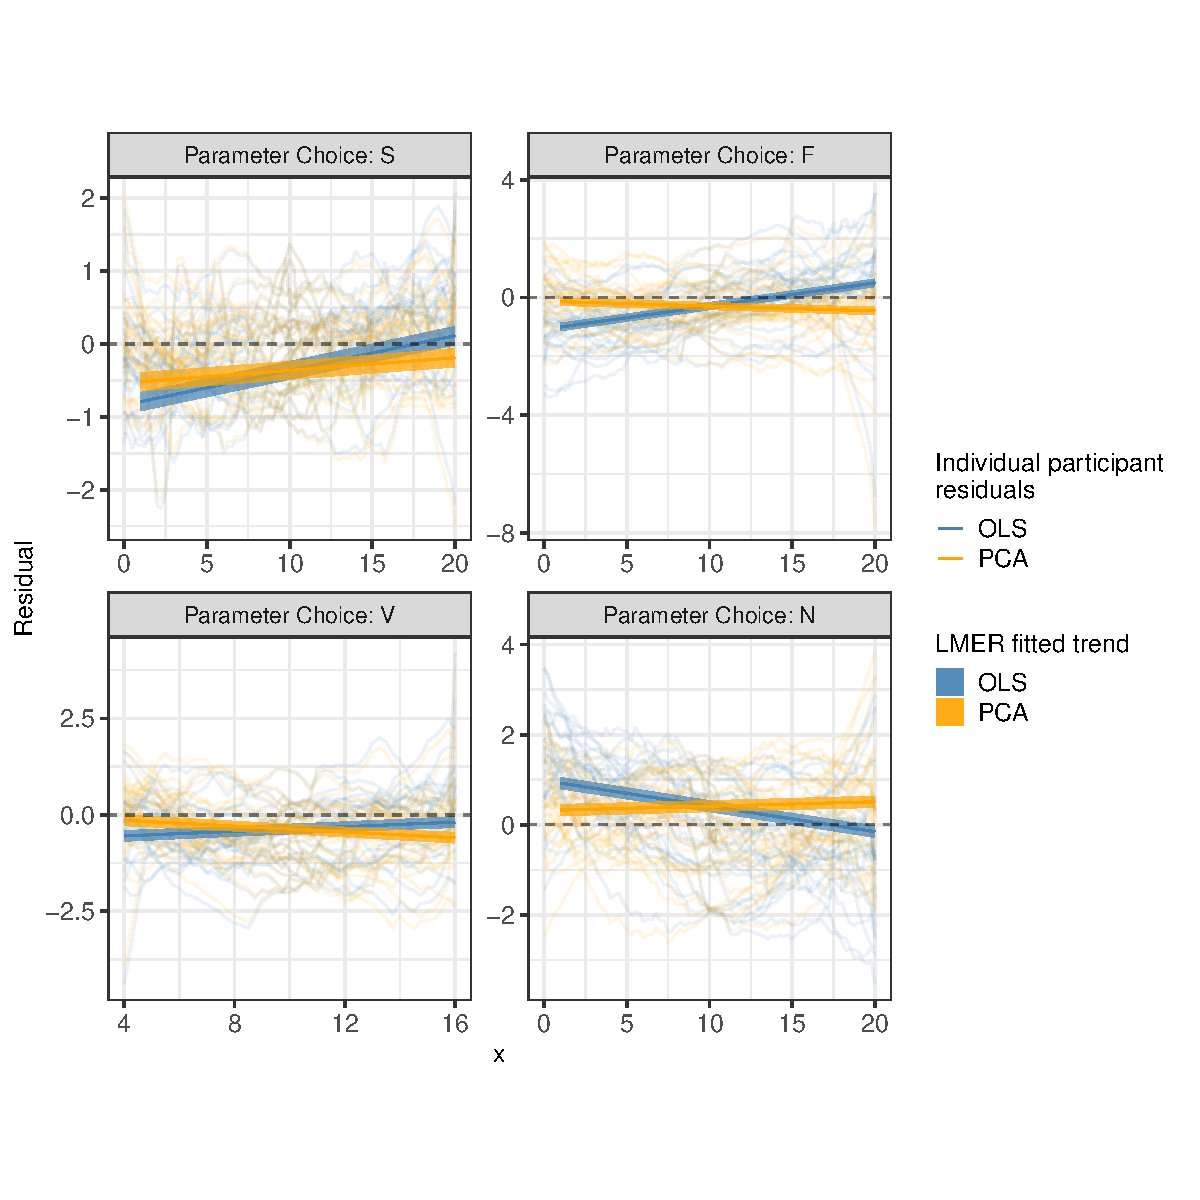
\includegraphics[width=0.9\linewidth,]{Eye-Fitting-Stright-Lines-in-the-Modern-Era_files/figure-latex/eyefitting-lmer-residualplots-1} 

}

\caption{Eye Fitting Straight Lines in the Modern Era LMM results}\label{fig:eyefitting-lmer-residualplots}
\end{figure}

\begin{figure}[tbp]

{\centering 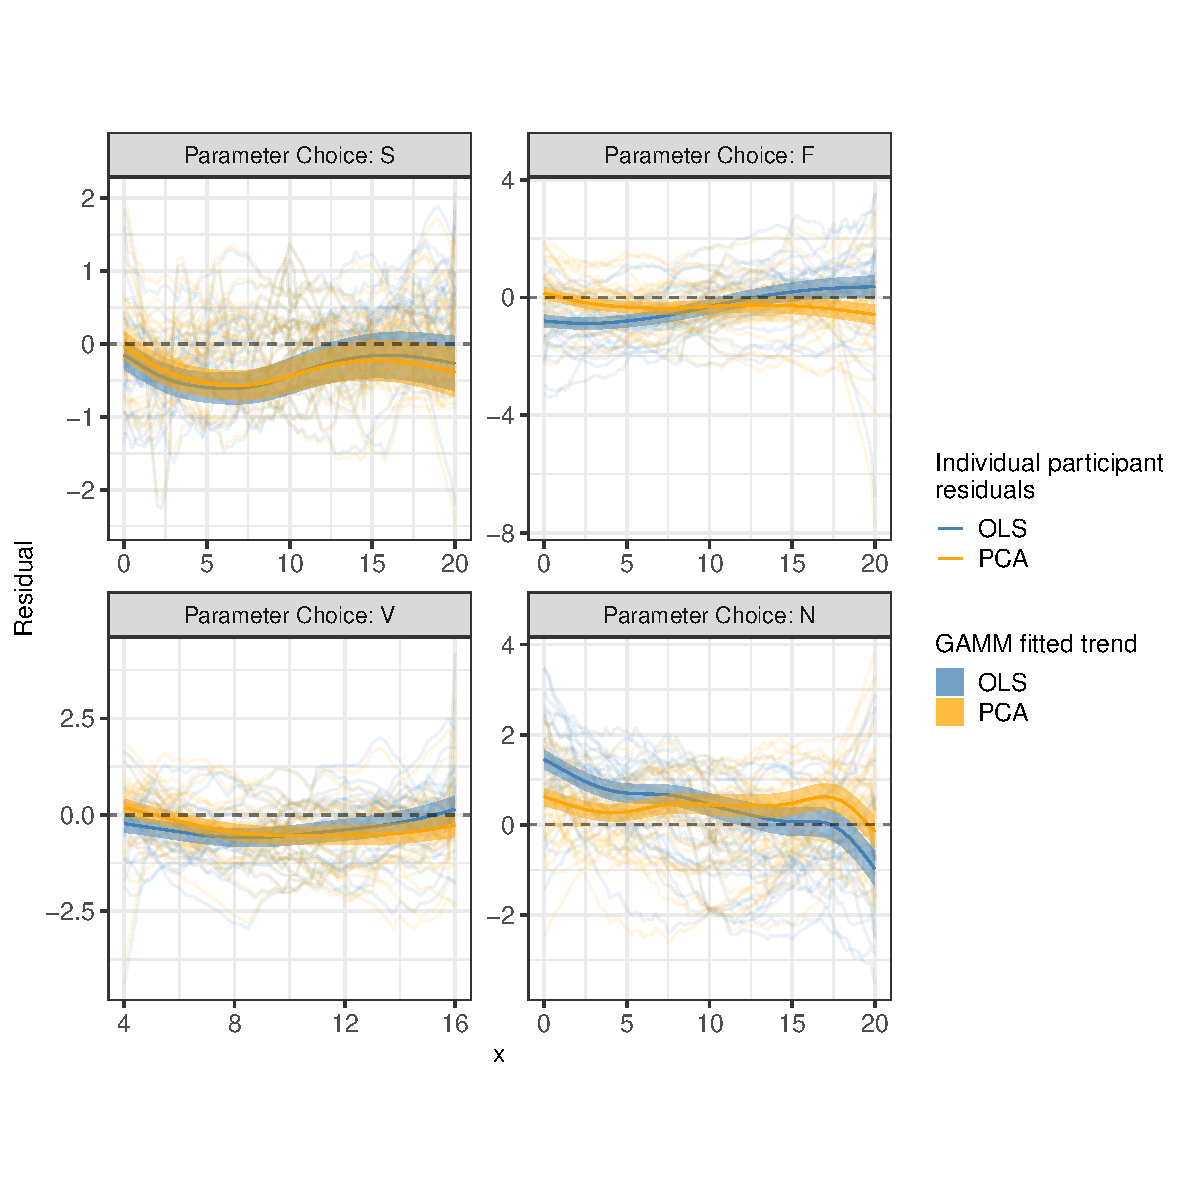
\includegraphics[width=0.9\linewidth,]{Eye-Fitting-Stright-Lines-in-the-Modern-Era_files/figure-latex/eyefitting-gamm-residualplots-1} 

}

\caption{Eye Fitting Straight Lines in the Modern Era GAMM results}\label{fig:eyefitting-gamm-residualplots}
\end{figure}

\hypertarget{discussion-and-conclusion}{%
\section{Discussion and Conclusion}\label{discussion-and-conclusion}}

The intent of this paper was to establish you draw it as a tool. Eye
Fitting Straight Lines in the Modern Era replicated the results found in
Mosteller et al.~(1981). When shown points following a linear trend,
participants tended to fit the slope of the first principal component
over the slope of the least squares regression line. This trend was most
prominent when shown data simulated with larger variances. The
reproducibility of these results serve as evidence of the reliability of
the you draw it method.

\hypertarget{future-work}{%
\section{Future Work}\label{future-work}}

Use the method. \emph{Should probably elaborate here..}

\bibliographystyle{agsm}
\bibliography{bibliography.bib}

\end{document}
